\chapter{Discussion}


\section{Reflection on the results}

Usability tests are important tools for the evaluation of a prototype. However, with a limited number of test persons, a quantitative analysis is not possible due to the necessity of a test group that is sufficiently large to produce statistically useful data. Even for a qualitative analysis, using the opinion of only one physical therapist may result in responses that are biased towards a certain view the therapist has on the subject. To distinguish between genuine design defects and problems only encountered due to individual bias, it is necessary to have a large enough test group. For the scope of this thesis, the number of user tests is limited, so a more careful approach is needed when interpreting the results of the test.\\

The test users, including the physical therapist, require time to get familiar with non-traditional gesture-based interface elements. The time needed depends on the person and his knowledge and experiences with other gesture-based interfaces. An important part of this is knowledge about the Kinect camera and its possibilities. The test users are worried of doing something that the application does not know how to process. A common problem is that it is unknown to the users that the Kinect can make a distinction between an open and a closed hand, even while there is visual feedback provided when opening or closing a hand: the hands on-screen turn respectively green or red. This means that the user does not consider opening or closing his hands when trying to interact with something on the screen. This problem is always related to the features supported by the used sensors. The Kinect camera supports this feature, but similar cameras may not. Because of this, it is not possible to simply assume user knowledge of this operation.\\

When test persons get the time to experiment with the interface at their own pace, they eventually find a way by themselves to interact with the application. Due to the limited amount of different interactive elements, the application has a gentle learning curve. A tutorial can help bringing new users up to speed with how to use the application. However, a tutorial can also be a source of frustration or confusion for the user if not done well. As such, tutorials should be seen more like a last resort instead of the go-to solution for any interface-related problem. More and better feedback and feedforward is generally the preferred option to choose, as it increases natural coupling between the required actions and its function. Also, providing redundancy concerning feedforward for an action can help make the interaction more clear as well. For instance, the color of an element changes when the users hovers over that element, implying that interaction is possible. This can be expanded by having a sound effect play at the same time the color changes.\\

A potential problem is the limited amount of space the user has in the room he is using the application. Unless the user is required to move left or right during the use of the application, all interactive elements must be placed within reach of the user's avatar. This means that non-interactive elements can be placed further away from the avatar. This introduces the problem of limited interface space on the screen and can result in elements that are functionally coupled together to be separated. For instance, the scrollbar with recorded gestures is on the right of the user's avatar, but the playback of the gesture is shown on the left. It limits the locational aspect of the functional feedback, but at the same time indicates that no specific action is required for interacting with the gesture display on the left as it is out of reach. For instance, to some extent, this can be compared to having to interact with a Blu-ray player, but receiving visual feedback from another place, i.e. the television screen.\\

Unrelated to the interface design, but an important part of the application is gesture recognition. Due to the chosen approach, it is possible to record and train gestures as as  moving gestures as well as postures. However, the way SVM works limits the requirement for high accuracy when executing a gesture or a posture. The executed gesture is always recognized as the recorded gesture that looks the most similar. If all of the recorded gestures are very dissimilar, gestures do not need to be accurately executed in order for them to be recognized as a specific gesture. This means that it is not possible to tell if a gesture is executed correctly. It requires the physical therapist to keep a close look at the way the patient performs a gesture during play.\\

Furthermore, the speed with which a gesture is executed is not checked. Only if the execution is too slow, it is not recognized as a recorded gesture. Faster execution does not affect the gesture recognition, on condition that the Kinect's sampling limitations are not surpassed. To solve this problem, as well as the previous problem of inaccurate executions, the therapist needs to record not only the required gestures, but also examples of how gestures should not be executed, i.e.\ gestures that are performed too slow, too fast or just not the way the gesture has to be done. This requires the therapist to record many examples of wrong executions, which requires a lot of time to do and eventually leads to a less pleasant experience during play as far fewer executions are accepted as being correctly executed. In addition, it requires the therapist to have some understanding of how machine learning works, which does not match the goal of designing an application that can be used without any programming knowledge.\\


TO DO: Add some binding text here. This was moved here from section 3.1.1.\\
A way to solve this problem is to predefine a specific gesture that activates the \emph{pointing mode}. In this mode, it is only possible to point to something on the screen or switch back to the \emph{gesture mode}. However, this gives more responsibility to the therapist, who has to remember what that specific mode changing gesture is and that he cannot input that gesture as a gesture for the patient. In addition, defining a preset gesture means that not every patient has the ability to perform it, as some may not be able to move an arm or a leg, for instance. Since, from an end-user point-of-view, this setup is confusing and undoes the application's elegance of simplicity, only games can be played that require only button presses as an input.


\section{Analysis using Wensveen's design framework \cite{Wensveen2004}}

Wensveen \cite{Wensveen2004} created a design framework that designers can use to make their product more tangible and interactive. Though his work was already discussed in chapter \ref{chapter: related work}, it is interesting to elaborate on the criteria he has set out and to look at the measure in which the UI design in this project fulfills these criteria.\\
The article states that the key to a more tangible and interactive interaction is by creating a natural coupling between the action that is performed by the user and its associated function in the program through feedback and feed forward. This can be done on six different aspects: time, location, direction, dynamics, expression and modality. A coupling in time can be achieved by having no delay between the action of the user and the feedback of the program, such as when pushing a button it changes color immediately. A location coupling is achieved by placing the feedback for the program in the proximity of the action of the user, in the previous example the button was coupled in time but also in location because the location where the user pressed was also where the feedback appeared. The direction is coupled when\textsc{} the feedback of the program moves in the same direction as the action of the user, such as a scrollbar that moves up when it is dragged up. A coupling in dynamics is achieved by giving feedback with the same position, speed, acceleration and force as the action of the user, for example, when dragging a scrollbar it follows the cursor with the same acceleration to the same speed so that the relative position of the cursor on the scrollbar doesn't change. Modality is a more abstract term that describes what a user expects to see, feel or hear when a certain action is performed. Wensveen explains modality by giving this example: "the touching of objects can cause a sound or moving an object can be visually perceived". So to couple action and function the feedback must react in a way that the user expects it to react based on his experience in the real world. To further clarify this we present the example of a slide button in an indent, the user expects the button to move within the indent when he drags it but he also expects it to stop at the end of the indent. The coupling in expression also needs some more clarification, what he means with a coupling in expression is that the feedback has a metaphorical link to the way the user performs the action or to the function to which the feedback belongs to. Wensveen's best example is that of the LED on an Apple Powerbook\textsuperscript{\textregistered}, he says "The light is an indication of the sleeping state of the system and has the same expression as a relaxed breathing rhythm". How this is interpreted in this thesis is made clear by the following example. On a Motorola Moto G\textsuperscript{\textregistered} 3rd generation with Android\textsuperscript{\textregistered} version 6.0.1, an overview of all the active apps can be shown, to close an app the user has to swipe it either left or right. The swiping expresses the act of throwing something aside because it is no longer needed which clearly links to the function of closing the app.

Each aspect can be coupled through three kinds of feedback or feed forward information: functional, inherent and augmented. Functional information is perceived when the activated function is actually performed, for example, the appearance of the letter "a" when the "a" keyboard button is pressed. Inherent information is feedback inherent to the medium that is used, such as the movement and clicking of a physical keyboard button when it is pressed. The previous examples were all examples of feedback, an example of inherent feed forward is the presence and shape of the "a" key on the keyboard indicates that it can be pressed. Augmented information is information that is added by the designer and is only bound to the action or function due to the context it appears in. For example, in most operating systems the progress of moving a file from one drive to another is indicated by a progress bar, this progress bar is not inherent to the function or the medium, it is only bound to the function by the context it appears in.

In his article, Wensveen already stated that a natural user interface (NUI), such as designed in this thesis, has almost no inherent information because there is nothing that the designer did not specifically add to inform the user of an action possibility or an action's effect, there is no physical object with which to control the NUI. The only true inherent information on a kinect is the presence and direction of the camera which indicates that something is registered in that direction. The original article always groups all augmented information together to make the link between action and functional information. In this situation there are two layers of augmented information, the information given by the puppet and the information given by the UI elements such as the rope and the scrollbar. How this works will become clear after the analysis of the puppet and the first UI element. The tool is best used to analyze every action with it's respective function separately,  but to keep this discussion relatively short only the connections between the user and the puppet, the puppet and the pulling of the rope, the rope and the start of the recording are discussed in detail and the rest is done in more general terms. All links described in the following sections are visualized in figure \ref{puppet_rope_framework}.

The coupling between the user and the puppet is very crucial because it is the user's way of interacting with other UI elements. If the puppet does not feel natural to the user, the rest of the interaction will also  feel unnatural.  The puppet is coupled to the user in time because there is no delay between the user's movement and the puppet's movement, the hand of the puppet also turns red immediately when the user closes the respective hand. Of course, this is only true when the computer is able to process the information fast enough, this is where the choice for a puppet over a schadow plays a major role as discussed in chapter \ref{chapter: design}. There is no coupling in location because the puppet is not near the same three dimensional location as the body of the user. The coupling in direction is strong because the puppet follows every move of the user though it breaks down when the user tries to reach down below.  The dynamics are coupled very well becuase the puppet's limbs make the\textsc{} same proportional and relative motion as the user so that the position, acceleration and speed are all proportional to the user's. The link in modality is weaker because there are many situations where the puppet differs from the user's reality, such as the limbs disappearing when the user moves out of the field of vision and the fact that the user cannot feel any of the UI elements that the puppet touches. There is also no expression because there is no metaphorical link between the action of the user and the puppet.

%user => puppet => augmented information:
%- time the puppet moves when the user moves with no delay, hand changes color when closed
%- no location the puppet's hand is not near the same three dimensional location as the hand of the user
%- direction the puppet's limbs move in is the same direction as the user, the only exception is when the user tries to bend down.
%- dynamics the puppet's limbs are make the same proportional and relative movements as the user so the position, acceleration and speed are all proportional.
%- no modality there are to many things that differ from reality such as limbs disappearing when they are out of the camera's field of view and limbs go over all of the UI objects
%- no expression there is no metaphorical link between the action of the user and the puppet.



The rest of the UI elements only interact with the puppet. They are represented in figure \ref{puppet_rope_framework} as the second augmented information block. The rope, as was seen in figure \ref{rope handle reaction}, to start a recording is coupled to the puppet in time because it changes color and moves only at those times when the puppet touches it. It is also coupled in location because it only changes around where the hand of the puppet is located. The coupling in both direction and dynamics is apparent because the rope moves downward with a downward move of the hand at the same acceleration and speed. Besides the fact that the rope can be grabbed like a real life rope, the coupling in modality is weak because it doesn't react to the user's touch with the same physics that a rope would. There is no link in expression because it doesn't matter how the puppet pulls the rope the effect is always the same.

%Puppet => rope for recording :
%- time it changes color or moves when the puppet touches it
%- location it changes color around where the hand touches the UI_element
%- direction it moves in the same direction as the hand of the puppet when grabbed
%- dynamics are coupled with those of the puppet because the element is fixed to the hand of the puppet.
%- no modality coupling is present, the rope only goes down for any other movement it does not react like a rope should
%- expression it turns red when grabbed, red is generally a signaling color 

The activated function, starting the recording, is only coupled in time with the rope UI element because it doesn't matter where, which direction, what speed the user pulls the rope, it will always result in the recording window appearing. There is however a more direct coupling between this function and the puppet, the record window appears on the location of the puppet.

\begin{figure}[H]
	\begin{center}
		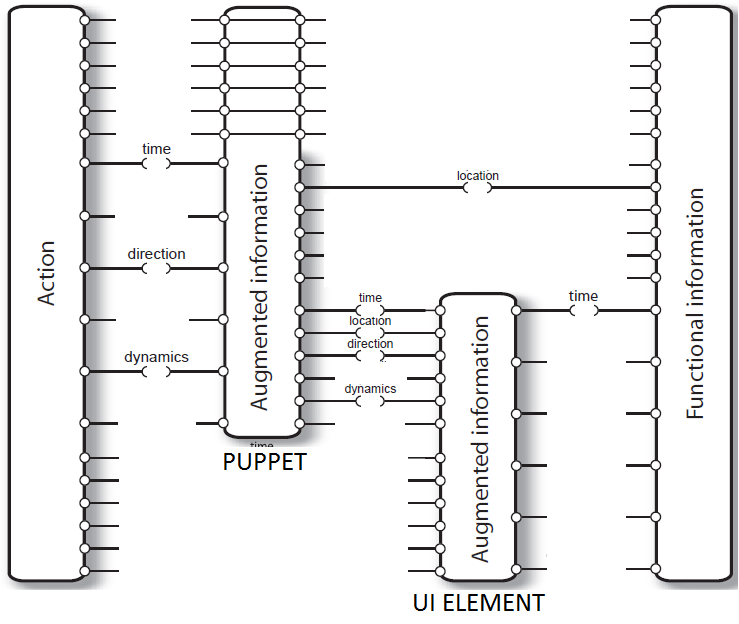
\includegraphics[width=14cm]{figures/standard_framework_Rope.png}
		\caption{\emph{Overview of the framework couplings for the puppet and the rope UI element}}
		\label{puppet_rope_framework}
	\end{center}
\end{figure}

The links from the user to the puppet stay the same for all of the UI elements, from puppet to UI element or function can be different. Assuming the computer can handle the workload, most of the UI elements are coupled in time with the puppet. a notable instance of time coupling is when the user wants to replay a recording as seen in figure \ref{replay of element six}, only when the puppet's hand hovers over the recording in the selection box area the recording starts to play. The change to green of the selection box is coupled to the puppet's hand in location, it makes the bridge to the replay screen because it also changes to green at the same time. The number of the recording is also shown on the screen at that time. The thorough link in time is because the coupling in location is so weak as mentioned before and no other couplings can be made. Both the scrolling and the delete slide have the same location, direction and dynamic coupling as the rope due to the general color coding and the fact that the movement of the UI elements are always the same as that of the hand that acts upon it. Though the delete action, seen in figure \ref{delete functionality}, has a special expression between the UI element and its function, the red color refers to signals like a red traffic sign or red traffic light that demand attention because they contain important information. 

%rope => open record screen
%- time it appears when the rope is pulled
%- no other links
%
%puppet => record screen 
%- location link the screen is drawn were the puppet stands.
%
%start recording
%
%end recording
%
%replay recordin
%- time has a strong link it only plays when the user hovers over it, same color, same number, 
%- location doesn't have a link it is far away
%- dynamics not really a link
%- no expression
%- no modality
%
%- 
%
%start scrolling
%- time when the puppet hoverover it green
%- location same time
%- direction follows hand
%- dynamics same dynamics as the hand
%-  no modality
%- no expression
%
%end scrolling 
%
%puppet => delete
%- time no delay
%- location hand over the middle of the object
%- direction follows hand 
%- no modality
%- red expression, delete fills with red expressing 
%
%
%
%
%link action to function: eloborate on what this means
%6 aspects that can do this: explain the exact meaning
%each aspect can have feedback and feedforward in 3 ways functional, augmented, inherent. give examples
%talk about the NUI only augmented feedback
%then talk about were our connection lay. and the reason why they are connected

\textsc{}
\subsection{part of literature to be added}
The idea to link gestures to keyboard button was conceived in a previous thesis \cite{Verbouw2016}


\section{Reflection on the process}

There are different approaches for designing an interface, but it always comes down to not treating the interface as an afterthought. As such, integrating the interface design right from the start with the back-end software design is essential. For instance, requirements concerning the responsiveness of the interface are for a big part set by the way the back-end software is designed and implemented. In other words, if the back-end is programmed inefficiently, this is reflected by a lack of responsiveness in the GUI.\\

However, it is necessary to switch fast from interface prototyping to an actual implementation. Since the early prototypes are static and non-interactive, it is only possible to really evaluate a decision after having an implementation of the concept and to obtain feedback from the users it is intended for. In other words, while static prototypes can undergo several iterations until they are \emph{perfected} in theory, only implementations in practice can really convey the feel of the interface.\\

To come up with ways of interacting with the application other than relying on traditional controls, an experimental approach is tested. The idea is to interview a physical therapist in order to obtain ideas from him concerning the interaction with the application. This makes it possible to find solutions that fit the needs and expectations of the user. Early tryouts of this experimental technique show that persons are reluctant of coming up with ideas they are not familiar with. It is more assuring and easier to fall back on traditional, well-known elements.\\

In the same sense, user testing often leads to results implying that more conventional interactive elements are easier and quicker to understand than others, even if they rely on making use of the mime pattern discussed before. This can be related to years of experience with other types of interfaces and confirms that there is need of a more streamlined way for gesture-based interaction that unifies all interfaces of this kind \cite{Norman2010}.\\

Including a scrollbar in a gesture-based interface is an example of this. The user has experience using scrollbars, so there are no problems to recognize the visual element as a list that can be scrolled through, but interacting with it is more difficult initially. This can be related to differences in the way gesture-based and touchscreen-based interfaces work. On touchscreens, it is possible to swipe with a finger on the screen to scroll, then lift it and touch the screen again to scroll again. With gesture-based interfaces, the action analogous to lifting the finger is less obvious to achieve. One way is to have the user move his hand out of the scrollbar before he can scroll in the same direction again. This is how it is implemented for the application. A different approach is to use composite gestures. The user can close his hand to grab the scrollbar and scroll through it, then open his hand, reposition it and close it to scroll again. This allows the action of scrolling to be faster, but it also adds the burden of having to remember more actions for interacting with this element and it can be tiresome to close and reopen the hand many times in succession. In the end, this comes down to personal preference and requires more user tests before a more general conclusion can be made.\\


\section{Future work}

Physical therapist Dries Lamberts indicated that the action of recording and training gestures can be pleasant for patients to do it themselves. This is especially useful if the developed application is not exclusively used for rehabilitation, but also as a way to have some physical exercise on a regular basis, as is the case for children with physical disabilities. As the GUI of the application is focused on being used by therapists, a different interface is required to simplify and optimize its use for children. This includes features like pressing a keyboard key to be designed appropriately.\\

A second possibility for future work is to use the current back-end structure to allow the user to create patient-specific projects, to which all gestures are coupled. On startup of the application, it can be possible to require the user to enter the name of a patient to load the project with all gestures they used before. This decreases the time needed before a patient can start exercising and playing a game.\\

Finally, the application can be expanded by adding screens to the interface that allow the user to manage different gesture classes and projects, reusing assets that are present in the developed interface.
